\section{Data and Experimental Setup}
\label{sec:setup}

\subsection{Datasets}

We use two public payment-fraud datasets that include a timestamp, which a chronological split requires (Table~\ref{tab:data}).

\textbf{IEEE-CIS} is the labeled portion of the data released by Vesta Corporation for the IEEE-CIS Fraud Detection competition~\cite{ieeecis2019fraud}. It consists of card-not-present e-commerce transactions covering about six months. Each transaction has an amount, a time offset in seconds, and several hundred anonymized card, address, device, counting and vendor-engineered columns. It is our main dataset because it is large and contains enough fraud cases to give stable estimates.

\textbf{ULB} is the credit card dataset released by the Machine Learning Group of Universit\'e Libre de Bruxelles~\cite{dalpozzolo2015calibrating}. It covers two days of transactions by European cardholders, described by 28 principal components, the amount and a time offset. It is short and contains few fraud cases, so every estimate on it is noisy, but it is one of the most widely used benchmarks and results on it are relevant to many published papers.

\begin{table}[htbp]
\caption{Datasets. The last two columns give the fraud rate in the first 80\% and the last 20\% of transactions in time order.}
\label{tab:data}
\small
\begin{tabular}{lrrrrrrr}
\toprule
Dataset & Transactions & Fraud cases & Fraud rate & Days & Features & First 80\% & Last 20\% \\
\midrule
IEEE-CIS & 590,540 & 20,663 & 3.50\% & 182 & 431 & 3.51\% & 3.44\% \\
ULB & 284,807 & 492 & 0.17\% & 2 & 29 & 0.18\% & 0.13\% \\
\bottomrule
\end{tabular}
\end{table}


Feature engineering is deliberately minimal, because the subject of the study is evaluation rather than leaderboard performance. We use the raw columns. Categorical columns are replaced by integer codes assigned in lexicographic order, which uses neither labels nor frequencies. The timestamp orders the data but is \emph{not} given to the models as a feature, because a raw timestamp could allow a model trained on a random split to memorize when fraud bursts occurred, and we did not want the main comparison to depend on that. Section~\ref{sec:mechanism} reports what happens when it is included.

\subsection{Split protocols}

\begin{figure}[htbp]
\centering
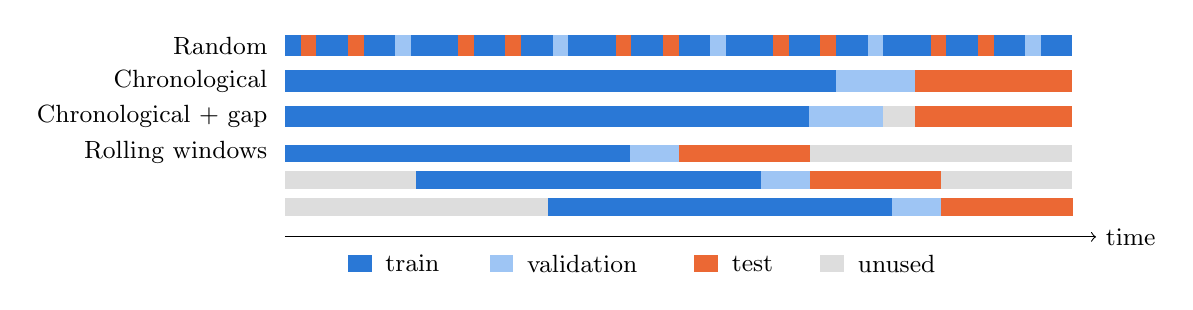
\begin{tikzpicture}[x=0.1cm,y=0.45cm,font=\small]
  \definecolor{tr}{HTML}{2A78D6}
  \definecolor{va}{HTML}{9EC5F4}
  \definecolor{te}{HTML}{EB6834}
  \definecolor{un}{HTML}{DDDDDD}
  % random: interleaved
  \node[anchor=east] at (-1,5.3) {Random};
  \foreach \i in {0,...,49} {
    \pgfmathsetmacro{\r}{mod(\i*7+3,10)}
    \pgfmathparse{\r<2 ? "te" : (\r<3 ? "va" : "tr")}
    \edef\c{\pgfmathresult}
    \fill[\c] (\i*2,5) rectangle ++(2,0.6);
  }
  % chronological
  \node[anchor=east] at (-1,4.3) {Chronological};
  \fill[tr] (0,4) rectangle (70,4.6); \fill[va] (70,4) rectangle (80,4.6); \fill[te] (80,4) rectangle (100,4.6);
  % gap
  \node[anchor=east] at (-1,3.3) {Chronological + gap};
  \fill[tr] (0,3) rectangle (66.5,3.6); \fill[va] (66.5,3) rectangle (76,3.6);
  \fill[un] (76,3) rectangle (80,3.6); \fill[te] (80,3) rectangle (100,3.6);
  % rolling
  \node[anchor=east] at (-1,2.3) {Rolling windows};
  \foreach \w in {0,1,2} {
    \pgfmathsetmacro{\y}{2-\w*0.75}
    \pgfmathsetmacro{\a}{\w*16.67}
    \fill[un] (0,\y) rectangle (100,\y+0.5);
    \fill[tr] (\a,\y) rectangle (\a+43.75,\y+0.5);
    \fill[va] (\a+43.75,\y) rectangle (\a+50,\y+0.5);
    \fill[te] (\a+50,\y) rectangle (\a+66.67,\y+0.5);
  }
  \draw[->] (0,-0.1) -- (103,-0.1) node[right] {time};
  % legend
  \begin{scope}[shift={(8,-1.1)}]
    \fill[tr] (0,0) rectangle (3,0.5); \node[anchor=west] at (3.5,0.25) {train};
    \fill[va] (18,0) rectangle (21,0.5); \node[anchor=west] at (21.5,0.25) {validation};
    \fill[te] (44,0) rectangle (47,0.5); \node[anchor=west] at (47.5,0.25) {test};
    \fill[un] (60,0) rectangle (63,0.5); \node[anchor=west] at (63.5,0.25) {unused};
  \end{scope}
\end{tikzpicture}
\caption{The split protocols. A random split interleaves training and test transactions in time, whereas the chronological protocols score only transactions that occur after every training transaction.}
\Description{Four horizontal bars over a time axis. In the random split, train, validation and test segments are interleaved. In the chronological split the first 70 percent is train, the next 10 percent validation and the last 20 percent test. The gap variant leaves the week before the test period unused. The rolling variant slides a train, validation and test window forward three times.}
\label{fig:splits}
\end{figure}


\begin{description}[leftmargin=1em,itemsep=2pt]
\item[Random.] A stratified random split into 70\% training, 10\% validation and 20\% test transactions (Figure~\ref{fig:splits}).
\item[Chronological.] Transactions are ordered by time. The first 70\% form the training set, the next 10\% the validation set and the last 20\% the test set.
\item[Chronological with a gap (IEEE-CIS).] As above, but the seven days before the test period are removed from the training and validation data. In production, the label of a transaction arrives only after a chargeback or an investigation, so the most recent transactions cannot be used for training~\cite{dalpozzolo2018credit}.
\item[Rolling windows (IEEE-CIS).] The six months are divided into six equal blocks. A model is trained on blocks $k$ to $k{+}2$ and tested on block $k{+}3$, for $k=1,2,3$. For each window we also draw a random split of the same four blocks with the same test-set size, so that the random-versus-chronological comparison is repeated on three different periods.
\end{description}

Under the random and chronological protocols, the final model is trained on the same number of transactions (80\%) and tested on the same number (20\%). The protocols differ only in \emph{which} transactions are assigned to each side.

The two test sets nevertheless differ, and a later period could simply be harder than an average one. We therefore add two controls in which both protocols are scored on the same transactions. The \emph{period-matched} control scores each random-split model only on those of its test transactions that fall inside the chronological test period. The \emph{blocked cross-validation} control compares five-fold cross-validation with random folds against five-fold cross-validation whose folds are five contiguous time blocks, so that each scheme tests every transaction exactly once. Blocked folds are not forward-looking, since a model may be trained on later data, but they remove the interleaving of training and test transactions in time, and the difference between the two schemes therefore isolates the effect of that interleaving.

\subsection{Models and tuning}

We evaluate five standard classifiers: logistic regression, a random forest~\cite{breiman2001random}, XGBoost~\cite{chen2016xgboost}, LightGBM~\cite{ke2017lightgbm} and a small multilayer perceptron (MLP). Table~\ref{tab:space} lists the search spaces.

Each model is tuned with 30 trials of Optuna's tree-structured Parzen estimator~\cite{akiba2019optuna}, maximizing \prauc{} on the validation set of the protocol at hand. The boosted models and the MLP use early stopping on validation \prauc{}. The selected configuration is then refitted on the combined training and validation data, with the number of boosting rounds or epochs found during tuning, and scored once on the test set. A seed repeats this entire pipeline, including the split (for the random protocol), tuning, refitting and testing, and we run five seeds. Under the chronological protocol the split is fixed, so the seeds vary only the tuner and the model. The standard deviations we report for that protocol therefore understate sampling uncertainty, and we complement them with a bootstrap over test transactions and with the rolling windows.

The tree models receive the raw matrix with missing values, and each tree of the random forest is grown on at most 100{,}000 sampled training rows. Logistic regression and the MLP receive median-imputed, standardized features with the amount log-transformed. The imputation and scaling statistics are computed on the training rows of each fit and never on validation or test rows.

\begin{table}[htbp]
\caption{Hyperparameter search spaces (30 trials per model, protocol and seed). $\alpha$ is the class-weight exponent of Section~\ref{sec:imbalance}.}
\label{tab:space}
\footnotesize
\begin{tabular}{ll}
\toprule
Model & Search space \\
\midrule
Logistic regression & $C \in [10^{-4}, 10^{2}]$ (log); $\alpha \in [0,1]$ \\
Random forest & 100 trees; depth $\in [4,24]$; minimum leaf size $\in [1,50]$ (log); feature fraction $\in [0.03,0.3]$; $\alpha$ \\
XGBoost & learning rate $\in [0.02,0.3]$ (log); depth $\in [3,10]$; minimum child weight $\in [1,50]$ (log); row \\
 & subsample $\in [0.5,1]$; column subsample $\in [0.3,1]$; $\lambda \in [10^{-2},10]$ (log); $\le$1000 rounds; $\alpha$ \\
LightGBM & learning rate $\in [0.02,0.3]$ (log); leaves $\in [15,255]$ (log); minimum leaf size $\in [10,200]$ (log); row \\
 & subsample $\in [0.5,1]$; column subsample $\in [0.3,1]$; $\lambda \in [10^{-2},10]$ (log); $\le$1000 rounds; $\alpha$ \\
MLP & 2--3 hidden layers of width 64, 128 or 256; dropout $\in [0,0.5]$; learning rate $\in [10^{-4},10^{-2}]$ (log); \\
 & weight decay $\in [10^{-6},10^{-3}]$ (log); AdamW, batch size 1024, $\le$30 epochs; $\alpha$ \\
\bottomrule
\end{tabular}
\end{table}

\subsection{Class imbalance and the oversampling leak}
\label{sec:imbalance}

The default treatment of class imbalance is cost-sensitive learning. The positive class receives weight $r^{\alpha}$, where $r$ is the ratio of legitimate to fraudulent training transactions and $\alpha \in [0,1]$ is tuned together with the other hyperparameters. A value of $\alpha=0$ corresponds to no weighting and $\alpha=1$ to full balancing.

A second experiment replaces class weights with SMOTE~\cite{chawla2002smote}, which synthesizes minority examples by interpolating between a minority example and one of its minority-class nearest neighbors. We run it in two ways under the random split.

\begin{description}[leftmargin=1em,itemsep=2pt]
\item[SMOTE on training rows.] The correct pipeline. Only the rows used to fit a model are oversampled, and validation and test rows are left untouched.
\item[SMOTE before the split.] The flawed pipeline described in some of the literature. The whole dataset is scaled and oversampled, and the balanced result is then split at random. Test rows are now half synthetic, and synthetic training rows have been interpolated from test fraud cases.
\end{description}

For the flawed pipeline we report two scores. The first is the score on its own oversampled test set, which is the number such a study would publish. The second is the score of the same fitted models on only the genuine transactions of that test set. The first score mixes two effects, a test set that no longer has the real class ratio and information flowing from test to training rows, whereas the second isolates the information flow.

On ULB the oversampling experiment uses the full data and five seeds. On IEEE-CIS, where oversampling doubles an already large training set, it uses a random subsample of 200{,}000 transactions and three seeds, with a class-weight baseline rerun on the same subsample. Rolling windows and cross-validation use one seed, since they already repeat the comparison over windows or folds.

\subsection{Metrics}

The primary metric is the area under the precision--recall curve (\prauc{}, computed as average precision), which is more informative than \rocauc{} when positives are rare~\cite{davis2006relationship,saito2015precision}. We also report \rocauc{} for comparison with prior work.

A fraud team can review only a limited number of alerts, so we additionally report \emph{alert-budget} metrics. The highest-scored 0.5\%, 1\% or 5\% of test transactions are flagged, and we measure \emph{recall}, the share of the test set's fraud cases that are flagged, and \emph{value recall}, the share of the fraudulent amount that the flagged transactions account for. Value recall weights each detected fraud case by its amount. The 5\% budget is included because fraud makes up more than 1\% of IEEE-CIS, which caps recall at the two smaller budgets.

\subsection{Implementation}

Experiments use Python 3.12 with scikit-learn 1.9~\cite{pedregosa2011scikit}, XGBoost 3.4, LightGBM 4.7, PyTorch 2.14~\cite{paszke2019pytorch}, imbalanced-learn 0.14 and Optuna 5.0, on a 14-core Apple M4 Pro laptop with 24\,GB of memory. The test scores of every run are stored, all tables and figures are generated from them, and code to reproduce every number is available at \ifanon a public repository (URL withheld for review)\else\url{https://github.com/mingwho/fraud-eval-time-aware}\fi.
